\chapter{Future Work Plan}
\label{chap:future}

We will be researching the \textit{why} of our approach for the next 10 months. In this time we will investigate the use of dependent types in our pure functional approach to agent-based simulation which we hypothesise should allow an unprecedented level of verification and validation, not possible (even not on a theoretical level) with imperative, traditional object-oriented approaches. There exists literally no research on this topic thus it will form the unique and sufficiently advanced, novel contribution of our PhD to the field. We will also write an additional paper which will investigate how dependent types can be made of use in ABS.
Around December 2018 I will start writing another paper which is targeted for an agent-based simulation journal and is written as a conceptual paper, describing the approach and benefits of purely and dependently typed agent-based simulation. While writing this paper I will start constructing the main argument structure of my thesis so I have structure already when I start writing the thesis in April 2019. The last 6 months of the PhD (April 2019 - September 2019) will be dedicated to writing up the thesis and conducting additional research if still necessary.

\begin{enumerate}
	\item Researching the HOW: September 2016 - March 2018
	\item Researching the WHY: April 2018 - March 2019
	\item Writing the Thesis: April 2019 - September 2019
\end{enumerate}

%2018
%August - September
%	research \& writing 3rd paper
%	holiday
%
%October - December
%	finalising research \& writing 3rd paper
%
%2019
%January - April
%	finalising and submitting 3rd paper
%	writing 4th paper: towards pure functional ABS. targeted for an agent-based simulation audience and written as a journal paper. this wont need any unique research but is basically a conceptual paper explaining my insights and research so far on a not too technical level to the ABS community - thus it is more about writing and not about unique research and programming, this has been done already at this point. this paper will help me very much in defining a basic structure of the thesis
%	defining structure of thesis
%
%April - August
%	writing thesis
%	publishing of papers
%
%September
%	holiday and moving to austria
%	submitting thesis


%Papers route: end of march 2018: PFE paper, dependent types in ABS: march 2019 for ICFP 2019, towards pure functional abs paper as concept paper to the ABS Community until april 2019 (before starting thesis writing) 

In this chapter we discuss in more detail how we plan to approach the aim and objectives stated in Chapter \ref{chap:aimsObj}. Further we give a short overview of planned papers and present a Gantt-Chart \ref{fig:gantt} reflecting the most important activities and relevant milestones.

\section{Approaching the Objectives: Dependent Types}
We have already begun working on dependent types and the plan is to do an in-depth research and examination of the ideas outlined in the section \ref{sec:dep_absconcepts} on the concepts of dependent types in Agent-Based Simulation.

Although there exists research on bringing dependent types to FRP \cite{sculthorpe_safe_2009}, we follow a fundamentally different approach in implementing ABS with dependent types. Instead of using FRP as described in section \ref{sect:how}, we follow the approach taken in the papers described in related work on dependent types \ref{sub:dep_abs_relwork}. The approach there is to implement a Monad, \textit{indexed} over additional parameters - in our case pre \& post state, time, environment boundaries,... - and write an interpreter for the operations the Monad supports.

The reason why we chose to follow a different approach was that we came to the conclusion that we would have to invest very much additional work to make dependently typed FRP work and that it would not allow us to encode the properties we want in types. Also it allows us to explore the other fundamental approach to program design in functional programming: implementing a \textit{shallow} encoded EDSL. Although it might seem that we are throwing a way a lot of work on \textit{how} to do ABS in pure functional programming, this is not so: the work described in section \ref{sect:how} was a very important step, getting us familiar with the concepts and approaches which will allow us to transfer a lot of insights. %The main difference will be that the system will most likely not be a continuous time-driven but an event-driven one, which allows us to explore even another route of implementation technique to ABS.

\paragraph{Implement SIR}
We implement an agent-based SIR model with an indexed monad, to explore the concepts described in section \ref{sec:dep_absconcepts} in the context of an explanatory model, which has an analytical background.

\paragraph{Implement SugarScape}
We implement the SugarScape model with an indexed monad, to explore the concepts described in section \ref{sec:dep_absconcepts} in the context of an exploratory model, which has no analytical background but follows hypotheses.

\paragraph{Extract Indexed Agent Monad}
After having implemented the dependently typed SIR and SugarScape we try to derive the common concepts into an indexed Agent Monad.

\paragraph{Total SIR}
The research on equilibrium and totality in the agent-based SIR model is a separate activity as we think that using indexed monads will probably not work for that approach and that we rather need to express relations in types from which the implementation will follow  .

\section{Planned Papers}
For the remainder of the Ph.D. we planned for two more papers.
The first one will be about applying dependent types to agent-based simulation and targeted towards a functional programming journal. We plan on start writing it end of the year around November / December 2018.

The second paper will be conceptual \textit{towards} paper which is basically a condensed version of all my research on pure functional programming and dependent types in Agent-Based Simulation and is targeted towards an agent-based simulation journal. With that paper we want to try to sell the concepts found in our research to the ABS community. We plan on start writing it around February 2019 as a precursor to start writing the thesis.

\section{Writing the Thesis}
I plan on start writing the thesis in April 2019 and hope to finish it at the end of the Ph.D. programme in September 2019.

\clearpage

\begin{landscape}
	\label{fig:gantt}
	\centering
	
	\begin{figure}
	\centering
	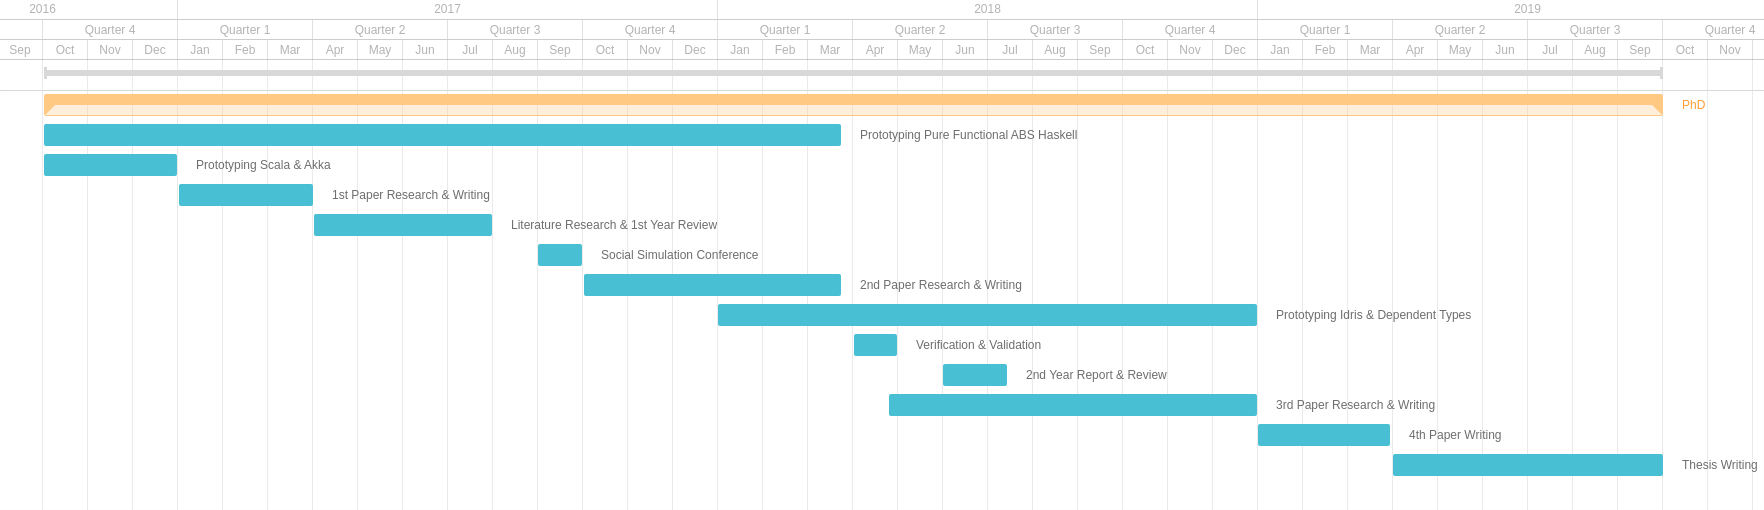
\includegraphics[width=1.5\textwidth, height=1\textwidth, angle=0]{./fig/phd_gantt.png}
	\caption{Gantt Chart of the Phd}
	\label{fig:gantt}
\end{figure}
\end{landscape}